\section{Depth-Based Tiebreaking for A*}

\label{sec:depth}

As shown in the previous section, the search spaces of Zerocost domains have many 0-cost edges,
resulting in a large final plateau ($\plateau{f^*,0}$). In a final plateau,
all nodes have $h=0$, so $h$-based tiebreaking cannot provide
useful guidance toward a goal. Thus, we need a new metric for discriminating among nodes
in the plateau so that the search algorithm can make progress in the plateau.

We define the \emph{depth} of a node as an 
integer representing the distance (number of steps) from the
\emph{entrance} of the plateau.  An \emph{entrance} of the plateau is
the first node which encountered in the plateau, along the path from the
initial node. These notions are depicted in
\refig{fig:plateau-depiction} (subfigure 1). 

\begin{figure}[htbp]
  \centering
  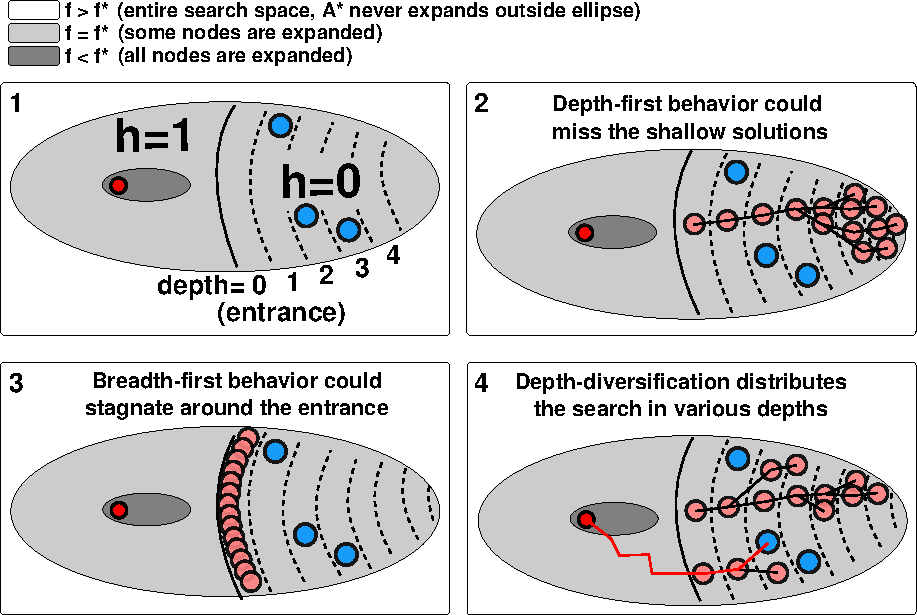
\includegraphics{img/astar/plateau-2.pdf}
 \caption{(\textbf{Subfigure 1}) The nodes in a plateau are divided into several layers, and each layer has the corresponding depth. Since all nodes have $f=f^*$, depth does not affect optimality. The goals in both shallower or deeper region yield cost-optimal solutions.
 (\textbf{Subfigure 2}) \lifo tiebreaking strategy results in depth-first behavior in a
 plateau, which could miss solutions if they are concentrated near the entrance.
 (\textbf{Subfigure 3}) \fifo tiebreaking strategy results in  breadth-first behavior in a
 plateau, which could fail to reach solutions in deeper layers within the time limit.
 (\textbf{Subfigure 4}) Depth-based diversification allows \astar to search the plateau space
 in a less biased manner. This balances exploration and exploitation, avoiding the problems with both \lifo (depth-first) and \fifo (breadth-first) behavior.
 }
 \label{fig:plateau-depiction}
\end{figure}

The depth $d(n)$ of a
node $n$ is 0 when $n$ and the parent node $m$ have different key
values for a sorting strategy, and $d(n)=d(m)+1$ when they have the same
key values: For example, in \astar with $h$-based tiebreaking, the key
values of a node are represented as a vector $[f,h]$, and they are same
when they are pairwise equivalent (i.e. $f(n) = f(m) \land h(n) =
h(m)$).  Having the same key values means that $n$ and $m$ are on the
same plateau.

The traditional \lifo and \fifo tiebreaking strategy 
search the plateau region in a decreasing and increasing order of the depth, respectively.
The \lifo strategy always selects the most recently generated node
within $\plateau{f,h}$, and the behavior in the plateau is equivalent to depth-first search.
Thus, \lifo always selects the largest depth
buckets, as depicted in \refig{fig:plateau-depiction} (subfigure 2).
Similarly, the behavior of the \fifo strategy 
in a plateau is equivalent to breadth-first search. Thus \fifo 
always selects the nodes with least depth (subfigure 3).
Note that  $[f,h,\lifo]$ is equivalent to $[f,h,-d,\lifo]$ and
$[f,h,\fifo]$ is equivalent to $[f,h,d,\fifo]$.

The problem with these traditional strategies is that we have no knowledge
regarding whether the goals are located close to or far from the entrance. Recall
that since $f=f^*$, all goal nodes in the final plateau are optimal with respect to solution cost
regardless of the depth.
%: A goal node in a shallower region or a deeper region both yields a cost-optimal solution. 
However, until we find a
solution, we do not know how the goals are distributed among various
depths. In some problem instances the goals can be concentrated around
the entrance, and in other problem instances the goals can be
concentrated at some large depth. % $k$.  k never used below?

In the former case, \fifo
should perform well because its breadth-first behavior naturally
focuses the search around the entrance favoring the smaller depths.
However, in the latter case, exhaustively searching
the shallower depths can result in not finding any solutions within
the time limit because \fifo may never reach the depth where the goals
exist.  On the other hand, \lifo behaves in a depth-fist manner, so it
may reach solutions at deeper depths quickly, but risks missing
solutions at shallower depths.  Thus, both \fifo and \lifo tiebreaking
are prone to failures due to pathological cases.

In order to avoid focusing the search at the wrong depths (too shallow/deep), 
the safest policy seems to be to simply \emph{diversify} the depths which are being searched,
in order to avoid any depth-based biases which could lead to pathological behavior.
In our proposed \emph{depth diversification} strategy, the nodes are inserted into buckets
associated with depths, and upon expansion, search effort is distributed in a more balanced manner
among various depths (\refsec{sec:theoretical-characteristics} defines ``more balanced''  more precisely).
Nodes are not  ``sorted''
according to increasing or decreasing order of depth -- instead, we try to 
``diversify'' the node expansion within the plateau.
We denote this depth diversification criterion as $\depth$. 
For example, $[f,h,\depth]$ first breaks ties according to $h$ values,
then uses the $\depth$ criterion to break ties in $\plateau{f,h}$.
%We denote such a diversification family of
%tiebreaking strategies by enclosing it in brackets such as $[f,h,\depth]$.

In order to diversify the expansion among depths, we simply
iterate over the depth buckets. An index $d_c$,
 which stores the depth (bucket index)  which was selected in the last expansion,
is initialized to 0.
At each expansion, the counter is decremented ($d_c\leftarrow d_c-1$) and
a node from  bucket $d_c$ is expanded. When $d_c$ reaches below 0, then $d_c$
is reset to the current largest depth in the plateau.

In an earlier, conference paper, we used a non-deterministic,
randomized implementation of this idea \cite{Asai2016}, but we use a deterministic
implementation here because it eliminates the possibility of results being influenced by random seeds,
and also facilitates the  theoretical analysis below in \refsec{sec:theoretical-characteristics}.

Depth-based diversification is significantly different from \ro the strategy which simply selects a random node from the OPEN list.
The uniform sampling behavior of  \ro behaves very similar to \fifo, and is insufficient to achieve the level of diversity provided by our depth diversification tiebreaking.
This is because at any given point in the search, more nodes will tend to have shallower depth than deeper depth, and a uniform, random selection will therefore be biased to select a node with shallow depth.
For example, imagine we have 100 nodes at depth $d=1$ and a single node at depth $d=2$.
Since \ro does not consider the depth, the chance of expanding $d=2$ is only $1/101$.
This probability does not improve until a sufficient number of expansions decreases the number of nodes in $d=1$.
In contrast, our depth diversification policy expands nodes at $d=1$ and $d=2$ with equal probability.


% We later show that
% \fifo and \lifo strategies are incomplete when the size of the plateau
% region is inifinite, while our \id is probabilistically complete.

%\subsection{The Scope Captured by Depth-Based Tiebreaking}
\subsection{When Does Depth-Based Tiebreaking Affect Node Expansion Order?}

% ``no effect'' is ambiguous, reviewers may complain that we are trying to claim there is no overhead, including the low level overhead. Thus I reworded from ``no effect'' to ``does not affect the order of expansion''.
Depth-based tiebreaking does not affect the order of node expansion when there are no remaining ties after the
higher priority tiebreaking criteria, in which case all nodes have depth 0. \todo*{mentioning ``keys'' seems
unnecessarily complicated, so remove it}
% 
This happens when the target problem only has operators with positive cost.
Let a node $n$ is a child of a node $m$. Depending on whether $n$ is already evaluated and whether the parent of $n$ is updated or not, there are 3 cases:

\begin{enumerate}
 \item If $n$ is evaluated for the first time,
       then $g(n)=g(m)+\mit{cost}(m,n) > g(m)$ and so $f(n)-h(n) > f(m)-h(m)$.
       Therefore, $f(n)=f(m)$ and $h(n)=h(m)$ cannot hold at the same time and the depth is 0.
 \item If $n$ is already evaluated as a child of another node $m'$, $n$'s current parent is $m'$ and
       $g(m)+\mit{cost}(m,n) < g(m') + \mit{cost}(m',n) = g(n)$,
       then the parent of $n$ is updated to $m$ and $g(n)\leftarrow g(m)+\mit{cost}(m,n)$.
       Since $g(n)=g(m)+\mit{cost}(m,n)>g(m)$ and so $f(n)-h(n) > f(m)-h(m)$,
       therefore $f(n)=f(m)$ and $h(n)=h(m)$ cannot hold at the same time and the depth is 0.
 \item If $n$ is already evaluated as a child of another node $m'$, $n$'s current parent is $m'$ and
       $g(m)+\mit{cost}(m,n) \geq g(m') + \mit{cost}(m',n) = g(n)$, then the parent of $n$ remains $m'$. If the
       depth of $n$ is 0 at this moment, then it remains 0 because the parent is unchanged.
\end{enumerate}

Since cases 1 and 2 always hold and case 3 holds at the beginning of the search,
by induction, case 3 always holds during the search.
Thus, the depths of nodes in positive cost domains are always 0.

\subsection{Tiebreaking within Depth Buckets}

Depth diversification cannot be a default tiebreaking by itself.
Consider a tiebreaking strategy such as $[f,h,\depth]$ which applies a depth-diversification tiebreaking.
After the $\depth$ criterion is applied, 
there may be multiple nodes within the same depth bucket, so a
default tiebreaking criterion is still necessary to break ties among them.
Thus, we should, for example, apply one of \lifo, \fifo or \ro (random order) criteria
after the $\depth$ criterion.

There are two concerns about this default tiebreaking criteria.
First, the default tiebreaking behavior is more prone to be
affected by the accidental biases, e.g., names/orders of action schema in the PDDL domain definition.
Second, in addition to accidental biases, there may be some nontrivial biases that require 
sophisticated algorithms to be removed.

Recent work  showed that the performance of satisficing
planner can be significantly affected by the order in which actions appear in a PDDL file \cite{vallati2015effective}.
However, the conference version of this paper \cite{Asai2016} showed that
the effect of such an accidental bias is not statistically significant in cost-optimal search,
by comparing the performance on
several sets of randomly ``mangled'' domains whose action names are replaced with random strings.
Moreover, the \ro default tiebreaking is supposed to be unaffected by such an accidental bias.
Thus, the experimental results we show in this paper is not a product of some piece of luck.

% ``breadth direction'' example was not well defined, replaced with vague discussion of symmetry (combined with the next par); also removing ``non-trivial'' because trivial/nontrivial is not obvious and undefined.
In addition to accidental biases, there may be other nontrivial biases such as some form of symmetry among states which can be removed using some tiebreaking criterion $X$.
Such a criterion can be applied after the depth criterion but before the default criterion,
resulting in a sorting strategy $[f,h,\depth,X,\fifo]$. 
Candidates for $X$ may
include pruning techniques such as Symmetry Breaking \cite{Fox1998,pochter2011exploiting,domshlak2013symmetry} or
Partial Order Reduction \cite{hall2013faster,wehrle2013relative}.
While they are usually described as ``pruning techniques'',
it can be rephrased as ``removing the bias to a set of similar/same nodes'' because
they both aim to prune the redundant nodes.
Note that redundancy causes a biased search effort. For example, imagine we have a
set of nodes $S=\{a_1, a_2, a_3, a_4, b, c, d\}$ where
$A=\{a_1, a_2, a_3, a_4\}$ are ``redundant'' according to some measure (e.g. by Symmetry,
Partial-Order). 
If a search algorithm expands $S$ by random selection, it favors the
group $A$ by giving 4 times larger chance of expansion than $b$,
$c$ or $d$.
Methods for addressing such biases is an avenue for future work.



\subsection{Theoretical Characteristics of the Depth Distribution}
\label{sec:theoretical-characteristics}

We give further insight into the search behavior of our implementation of depth-based diversification.
In the diversification, although the random selection from the depth buckets is possible,
our implementation performs a deterministic, round-robin sampling from the available depth buckets as described above.
%iterates from the largest depth to 0.
% 
%We are particularly interested in how the expansions happen among the
%various depths in the plateau region.
We are particularly interested in how the nodes selected for expansion are distributed 
among the various depths in a plateau region.
Using a simplified model where the plateau region forms a forest (a set of disjoint trees),
we can analyze the number of expansions in a particular depth
can be represented by a simple formula. 
% Although the notion of
% probability does not fit well with deterministic \fifo or \lifo
% default tiebreaking, it is still meaningful in the case of \ro (random
% order) default tiebreaking.

%% danger!!
% \begin{theo}[Uniformness of the search]
%  Assume the search space forms a forest of fixed width $w\geq 2$.
%  After enough number of iterations $D$,
%  the chance of expanding each node is unaffected by the depth of the
%  node, if the depth $d$ is small relative to $D$.
% \end{theo}

% I no longer claim the distribution is uniform.

% As a preparation, we first show that the number of expansion happened to each depth decreases
% linearly with the depth.

% 
\todo*{Introduced the forest assumption in the beginning.}
In the discussion below, we assume the following.
First, we assume that the plateau region forms a forest of a fixed branching factor
$w\geq 2$ (\emph{forest assumption}), rather than a graph with an indefinite number of successor nodes.
In the later experiments, we show this assumption is not much distant from the real situations.
Also, we assume that no depth bucket exhausts due to the expansion (\emph{no-exhaustion assumption}).
We provide a condition for this assumption to hold within this section.
% Finally, we assume that the sorting strategy performs a \ro default tiebreaking
% after the depth-based diversification is applied.

Let $D\geq 0$ be the current largest depth of the nodes found in the plateau so far. An expansion of a node in
depth $D$ results in more nodes on the same plateau, which have depth $D+1$.  Due to the forest
assumption, these children are all newly generated. Also, as we explained in the previous section, the expansion is
diversified by a sequence of iterations from the current largest depth to 0.  It means that when the current
largest depth of the plateau is $D$, the number of iteration executed so far is also $D$ because
in each iteration the largest depth is increased by 1.
% Under the forest assumption, each expansion of depth $d$ results in $w$ new nodes in depth $d+1$. 
Therefore, at the end of the $D$'th iteration, each depth $d$ has been expanded exactly $D-d$ times, with $D(D-1)$
expansions in total.

It also means that a sufficient condition for the \emph{no-exhaustion assumption} to hold until the end of the $D$'th
iteration is that the initial number of nodes in depth 0 is at least $D$.  If there are at least $D$ nodes in depth
0, depth 0 is trivially never exhausted until the $D$'th iteration. Also, no depth buckets in depth $d>0$ will be exhausted 
because each bucket has $w(D-d+1)$ generated nodes in total (i.e. OPEN+CLOSED) while the expansion has
happened only $D-d$ times.
The number of nodes in each bucket ($w(D-d+1)$) follows from the fact that  depth $d-1$ is expanded $D-(d-1)$ times in the preceding $D$ iterations.
Since $w\geq 2$, $w(D-d+1)\geq 2(D-d)+2>D-d$.
% For simplicity, let us also assume that the depth 0 initially have exactly $D$ nodes and
% no nodes will be added to depth 0 during the search.
% Also let $N=w(D-d+1)$ for readability.

Under our assumptions,  this distribution is an invariant which holds at any point of the search
until the solution is found. In fact, every depth-selection criterion, including the least depth selection (\fifo) or
the largest depth selection (\lifo), expands the same set of nodes if there are no solutions (each depth
$d$ is expanded $Dw^d$ times) and results in the same distribution.
However, their online characteristics are different.
For example, in \fifo, all nodes with $d<D-1$ are expanded while depth $d=D-1$ can take an arbitrary number of expansions $e \in [0, Dw^{D-1}]$ and depth $d=D$ is not expanded at all.
Also, in \lifo, for some $k\in [1,D_\mit{max}]$ (assuming the forest has a finite maximum depth $D_\mit{max}$), there can be a situation where all depths $d \in [0,k]$ gets only 1 expansion
while all nodes in depths $d \in [k+1,D_\mit{max}]$ are expanded. In this case, the number of expansions in $d \in [k,D_\mit{max}]$ is exponential to $D_\mit{max}-k$ ($\sum_{i=k}^{i=D\mit{max}}w^{i-k}=\frac{1-w^{D\mit{max}-k+1}}{1-w}$) while the number of expansions in $d \in [0,k-1]$ is linear to $k$ ($k-1$). Such an imbalance during the search causes the pathological behavior mentioned above.

\todo*{maybe \lifo and \fifo should be analyzed wrto this forest model and compared directly to each other as well as
$\depth$?}
\todo*{less priority -- lets add it when required by the reviewers. unused texts are in unused/lifo-fifo-distribution.tex}

